% ------------------------------------------------
%-------------------------------------------------
% Created by Ryan Sharp u1090072
% CSC3600 - Final Report
% Due 17th of October 2019
% ------------------------------------------------
% ------------------------------------------------

% ----- Include ----- %
\documentclass[11pt]{article}
\usepackage{graphicx}
\usepackage{amssymb, amsmath}
\usepackage{multirow}
\usepackage{graphicx, color}
\usepackage{wrapfig}
\usepackage{float}
\usepackage{changepage}

\setlength{\parindent}{0pt}

\begin{document}

% ----- Start Title Page ----- %

    \begin{titlepage}
        \centering
        \vspace {1cm}
        \huge{\textbf{CSC3600 Final Report}} \\ [0.1cm]
        \begin{figure}[ht!]
            \centering
            \def\svgwidth{0.5\columnwidth}
            
\includegraphics[scale={0.20}]{USQ.jpg}
        \end{figure}
        \vspace {0.5cm}
        \Large{By} \\
        \Large{\textbf{USQ Learning Emporium}} \\
        \Large{Richard Dobson, Jesse Hare, James McKeown, Vincent Roberts, Ryan Sharp} \\[0.50cm]
        \Large{Examiner} \\
        \Large{\textbf{Dr. Xiaohui Tao}} \\
        \Large{\textit{Senior Lecturer (Computing) – School of Sciences -
PhD QUT}} \\[0.50cm]
        \Large{Project Supervisor} \\
        \Large{\textbf{Assoc. Prof. Stijn Dekeyser}} \\
        \Large{\textit{Associate Professor (Computing) - School of Sciences - PhD Antwerp}} \\[0.50cm]
        \Large{School of Management and Enterprise} \\[0.50cm]

        \Large{Due: Friday 18th of October 2019}
    \end{titlepage}


\newpage

% ----- End Title Page ----- %



% ----- start ToC ----- %

\tableofcontents
\newpage

% ----- start ToC ----- %





\setcounter{secnumdepth}{0}
% ----- Section 1 ----- %

\section{1. Executive Summary}
This report provides an analysis and evaluation of the development stages completed for the harvest metadata.

\newpage



% ----- Section 2 ----- %

\section{2. Methodology}

\subsection{2.1 Methodology Statement}
The team used the scrum implementation of the agile methodology to complete the project. The scrum process allowed the team to incrementally build the program over the entire project duration. As there was constant input from the the project supervisor and the client, the scrum process permitted the team to make quick changes.

\subsection{2.2 Justifications}
The following sub sections will describe why scrum was chosen, the benefits of scrum and the disadvantages of scrum.

\begin{adjustwidth}{1cm}{}

\subsubsection{2.2.1 Why Scrum Was Used}
As stated in the previous section, scrum was ideal for this project as it allowed the team to make quick changes during the development process. Another reason why scrum was chosen was because there was no team leader. This provided an environment where all team members could be equal and address issues as a whole group. 

\subsubsection{2.2.2 Benefits of Scrum}
Scrum provided a framework that allowed the team to build in sprints, which suited this type of project. After each sprint, a meeting with the project supervisor was organised so that feedback could be given in preparation for the next sprint. In addition to this, scrum forced the team to prioritise requirements which allowed for faster development. Without this, lower-priority requirements may have been implemented at the cost of the higher-priority requirements.

\subsubsection{2.2.3 Disadvantages of Scrum}
As time constraints were a major factor in the development of the project, it was difficult for the team to have as many daily meetings as scrum required. Scrum requires the implementation of daily meetings, which wasn't feasible with this project. Another disadvantage with scrum in the team's case, was that each member of the team wasn't experienced with the process and the roles involved. This meant that the roles outlined in the scrum process weren't followed 100\% correctly.

\end{adjustwidth}

\subsection{2.3 Discussions}
The following sub sections will discuss how the scrum process was utilised and how it will be used for future projects.

\begin{adjustwidth}{1cm}{}

\subsubsection{2.3.1 How Scrum Was Followed}
All team members simulated the \textit{Product Owner} and \textit{Scrum Master} roles. Due to the inexperience with scrum, it was decided that this was the best option to follow. Daily meetings were reduced to at least 1 meeting a week, with 2 meetings a week the average throughout the duration of the project. Sprints were carried out every 1 to 3 weeks, depending on the size of the individual tasks. Once a sprint was complete a whole team meeting was organised to discuss the next sprint. Meetings were then held with the project supervisor to demonstrate what had been completed and to gain new requirements for the project. 

\subsubsection{2.3.2 How Scrum Will Be Used In The Future}
The obvious improvement to the scrum process in future projects would be to have a dedicated product owner and scrum master. These two roles play a key part in the scrum process, and when included, make the development of the project a lot easier. In addition, having more time to have daily meetings would help tremendously in both planning and developing the project. \\

Due to this being the first time each member had used the scrum process, it can be presumed that it wasn't as efficient as it could have been. As with all projects of this nature, the more experience you have, the faster and more efficient you get. It is the goal of all members, that with each time they use the scrum process they get more proficient with using it.

\end{adjustwidth}


% ----- Section 3 ----- %

\section{3. Project Process}

\subsection{3.1 Team Organisation}
There were a total of 5 members in the USQ Learning Emporium team. As this project was initially designed for teams of 3, the team needed to strategise ways in which to divide the work evenly between members. The first solution was to divide the main project task into 2 sub teams; a back-end team (3 members) and a front-end team (2 members). Within these teams each member had different roles. \\

From these sub teams, each had their own Facebook Messenger group and their own Slack channel for discussing specific project tasks. This stopped unnecessary information from being communicated between the sub teams, i.e. the back-end team didn't need to know the specifics of the front-end and vice versa. Within these messenger platforms, jobs were distributed and agreed upon between members.

\subsection{3.2 Team Structure and Roles}
As stated above, the group was divided into 2 main groups;  a back-end team (3 members) and a front-end team (2 members). The back-end team consisted of: James McKeown (Team Leader), Richard Dobson (Programmer) and Vincent Roberts (Programmer). The front-end team consisted of: Jesse Hare (Team Leader), Ryan Sharp (Programmer). \\

James McKeown and Jesse Hare both lead their respective teams. This allowed for better and more effective team co-ordination. It helped all members stay on task and stopped individual team members from deviating from the plan and doing their own work. Both of these members (James and Jesse) took on the most technical aspects of the project, especially in regards to the planning the project (in terms of coding). Other members then utilised this research to program their respective tasks within the project. 


\subsection{3.3 Communication and Meetings}
The following sub sections will discuss how well the team communicated throughout the project duration.

\begin{adjustwidth}{1cm}{}

\subsubsection{3.3.1 Effectiveness of Communication}
Communication between members was very quick and effective. The team decided to use a private Facebook Messenger chat as the primary point of contact as each member regularly used this application. This made it easier to notify team members of urgent matters. In addition to Facebook, the team decided to use a Slack channel for more technical and project specific subjects. Slack was new to all members and was therefore not utilised to it's full potential. \\

The main problem faced with the Facebook Messenger chat, was that the information couldn't be organised. It would have been better to use Slack as the primary messenger application as it was more suited to this type of project; especially because we had 5 team members and 2 sub teams. In future projects organisation of information needs to be a higher priority.

\subsubsection{3.3.2 Team Meetings}
Team meetings were run through the Zoom video conferencing application. At least once a week the whole team would meet to discuss the progress of the project. Meetings for the back end and front end team were often held more than once a week to discuss new ideas for their respective tasks. These meetings were highly effective as each member could screen share what they were working on and clearly communicate that with the team. \\

These meetings could be improved by having a set agenda before each meeting. Occasionally the meetings started slow as we all had to organise what we were going to discuss. It would also be ideal to have one member as the designated scribe to take notes for each meeting and relay this back to the team.

\end{adjustwidth}

\subsection{3.4 Documentation}
The activity log sheets, task summary sheets and meeting minute documents all assisted in tracking how the project was developing. The activity log sheets provided a good point of reference each week in deciding what tasks needed to be worked on next. It also helped ensure that each task was completed. Without the activity log sheets and task summaries it would have been difficult to keep track of the progress of the project. However, it was often the case that some weeks would be forgotten and team members would need to go back and fill in the information. This was obviously not ideal, but did not have a noticeable effect on the productivity of the team. \\

The meeting minutes documents were essential for the project. Without them, members of the team would forget what was discussed in each meeting. This would result in a massive amount of lost time as information would need to be repeated. After each meeting with the project supervisor (Stijn Dekeyser), the team would stay back and document what had been discussed in these meetings. This helped tremendously when working on specific parts of the project. This is because we now had a reference to look at, to see if certain features needed to be implemented. These meeting minutes can be found attached to the bottom of this document.


\subsection{3.5 Process}
The following sub sections will discuss the process used to develop the project, the difficulties encountered with this process and beneficial strategies used throughout the project duration.

\begin{adjustwidth}{1cm}{}

\subsubsection{3.5.1 Overall Process}
The team (and it's sub teams) decided on using the agile methodology for the project. Each week a meeting was held between members to discuss what tasks needed to be completed that week. Every 2 - 3 weeks a meeting was held with the project supervisor to discuss improvements that needed to be made. These improvements (as tasks) were added to the list of tasks to be completed.

\subsubsection{3.5.2 Difficulties Encountered}
Due to time constraints, university commitments and conflicting schedules, some weeks were more challenging than others. As a result some tasks did not get completed on schedule. This resulted in the rescheduling of tasks which hindered productivity. Any difficulty faced was getting team members  schedules to align. Occasionally, tasks would get worked on individually and passed on to another team member. Ideally in the real world, each member would have this project as their number one priority with no external distractions (such as university commitments, work etc.).

\subsubsection{3.5.3 Beneficial Strategies}
Weekly video conference meetings were essential for the project completion. These meetings allowed each member to discuss, and show, exactly what they were working on. Especially as the group implemented the agile methodology, it was important to discuss any improvements to the project each week. \\

Using Trello boards also assisted in the development of the project. It allowed all of the tasks to be laid out for each member to see. Once a task was completed it was moved from the 'to-do' card into the 'completed' card. As there were 5 members of the team, it was extremely beneficial as the tasks could be marked as 'to-do', 'doing' and 'completed'. This helped in reducing and avoiding work that would otherwise be repeated.

\end{adjustwidth}


% ----- Section 4 ----- %

\section{4. Project Report}
\subsection{4.1 Project Outcome}
Lorem Ipsum

\subsection{4.2 Cost of the Project}
The following sub sections will discuss the time and labor costs of the project.

\subsubsection{4.2.1 Cost of Hardware}
There are no deviations to the cost of hardware from the projection provided in the initial project plan. The costing table can be viewed below. \\

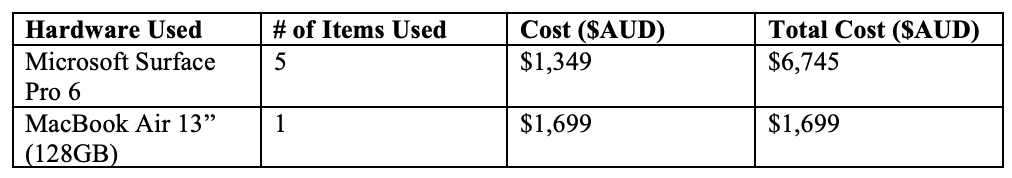
\includegraphics[scale=0.71]{hardware_table.png} \\


As the project was worked on remotely, all team members required company issued equipment. There were a total of 5 Windows machines provided to each member, with an additional MacBook Air provided to the project leader, James McKeown. There were no unexpected circumstances that required the purchase of any other pieces of hardware.

\subsubsection{4.2.2 Cost of Software}
There were multiple software solutions that were incorporated for the development of the project. There were some software solutions that were not foreseen in the initial project plan. All of the software solutions can be viewed below. \\

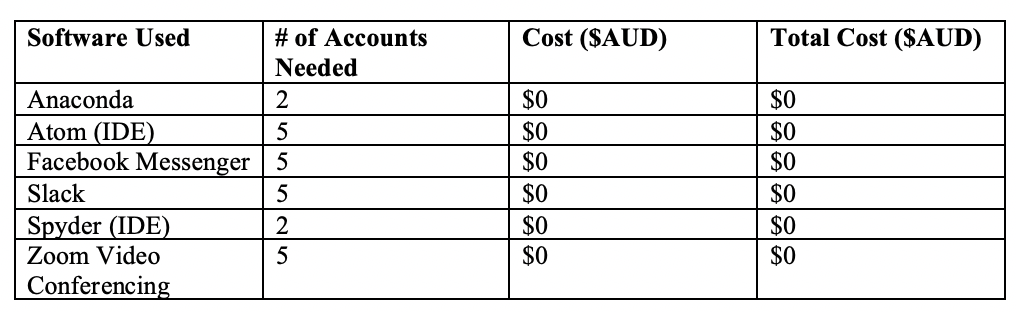
\includegraphics[scale=0.71]{software_table.png} \\

In the planning stages it was decided the front-end team would use Spyder as the preferred IDE. It added more specific functionality compared to Atom in our case. Anaconda was also used for the development of the front-end GUI. Facebook Messenger and Slack were used for communication between team members. Zoom Video Conferencing was used for group meetings and screen sharing. \\



\subsubsection{4.2.3 Time Cost}
The project took 12 weeks to complete with each member contributing 20 hours a week. Each member therefore contributed 240 hours of work to the project with a combined team total of 1,200 hours.

\subsubsection{4.2.4 Labor Cost}
The team was split up into 2 sub teams, a front-end team and a back-end team. The front-end team consisted of Jesse Hare and Ryan Sharp. The front-end team consisted of James McKeown, Richard Dobson and Vincent Roberts. \\

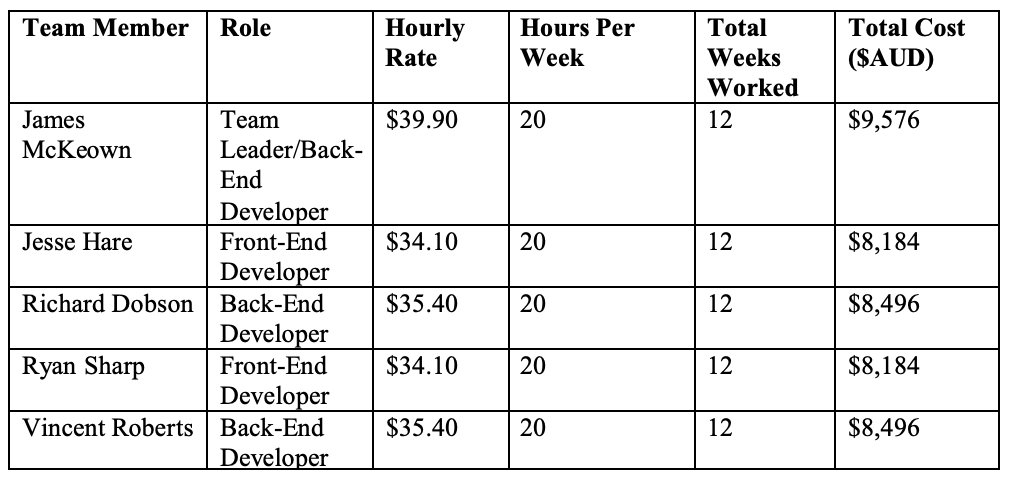
\includegraphics[scale=0.71]{team_cost.png} \\

The only difference between the projected labor cost and the actual labor cost was the error in how many weeks the project would take. It was initially predicated that the project would run over 10 weeks, when in fact the project ran for a total of 12 weeks.

\subsubsection{4.2.5 Lessons Learnt About Project Cost Estimation}
The major lesson learnt was that no prediction about the cost will be 100\% accurate. Lots of things change in a 12 week period and there is no possible way that these can be accounted for. For example, majority of team members used Atom before this project, so it was assumed that we would use this again. However, once the front-end team researched more into what programs were out there, it was decided that Atom was not the idea choice and that the team should use Spyder instead.


% ----- Section 5 ----- %

\section{5. Professionalism and Professional Ethics}

\subsection{5.1 Professionalism}
Throughout the project, professionalism was kept to a relatively high standard. In future projects, it would be optimal to have a set of professional standards that outlines what is expected of each team member. This would allow the team to refer back to this document should any breach of the standards occur. The following sub sections will discuss issues related to professionalism that occurred during the project.\\

\begin{adjustwidth}{1cm}{}

\subsubsection{5.1.1 Client Interaction Confusion}
Client interaction is the most important part of a project, without them the project would not exist. In this project, the client was also the project supervisor who gave information on behalf of both parties. While this did not have a major effect on the outcome of the project, it was obviously difficult to differentiate between a client meeting and project supervisor meeting. As a team, we should have been clearer with the meetings we wanted to have. Upon reflection, it would have been better if we clearly communicated they type of meeting we would like with the project supervisor. 

\subsubsection{5.1.2 Lack of Client Interaction}
It is important for any project to get as much client input as possible too ensure client satisfaction. While the team met the required amount of meetings with the client, it was most likely not enough. In a real world scenario it would have been best to meet with the client every 1 to 2 weeks, especially as the scrum process was used. This would have ensured that at every sprint the client had some input into the project and could see updates regularly. 

\subsubsection{5.1.3 Team Communication}
Communication between team members is essential for the progress of a project. On occasion, some team members did not reply to messages in a timely manner. This effected the progress of the project as some work had to be delayed to due other work not being completed. This was addressed via a team meeting, where all members gave their opinions on the matter. The issue was addressed and after the meeting took place, this particular issue did not happen again.

\end{adjustwidth}

\subsection{5.2 Professional Ethics}
Throughout the project professional ethics was also kept to a relatively high standard. As this project was conducted in a university environment, and was therefore a mock real world project, there were some professional ethic concerns. These will be discussed in the following sub sections.

\begin{adjustwidth}{1cm}{}

\subsubsection{5.2.1 Sharing of Sensitive Client Information}
Data privacy should be top priority for any business and business project. Due to financial constraints of the project is was not feasible to have a private GitHub repository. This resulted in the team using a public GitHub repository that could be accessed by any member of the public. In a real world scenario this would be very bad practice. In future projects, with more financial backing, it would be essential that private GitHub repository be used.

\subsubsection{5.2.2 Issue 2}



\end{adjustwidth}

% ----- Section 6 ----- %

\section{6. Contribution Distribution}

\subsection{6.1 How Work Was Distributed}
Each sub team, front-end and back-end, were responsible for their own individual tasks. Meetings were held on a weekly basis to decide what tasks needed to be completed that specific week. These tasks were allocated to team members based on their previous knowledge and experience of the task. For example, Jesse had previous experience with some Python GUI elements, so he was tasked with researching and developing the initial concept.


\subsection{6.2 How Effective Was The Distribution}
This method of distributing tasks worked quite well and resulted in a clear structure that needed to be followed. Without this distribution, team members would be going off and doing there own thing. This way each member knew exactly what they needed to do. While distributing tasks, there was no way to make sure everyone received the same amount of work. This was the only hurdle faced, but was mitigated as best best as possible.

\subsection{6.3 Task Distribution Table}
The following table represents the tasks completed in the project and the percentage of effort put it in by each team member. \\

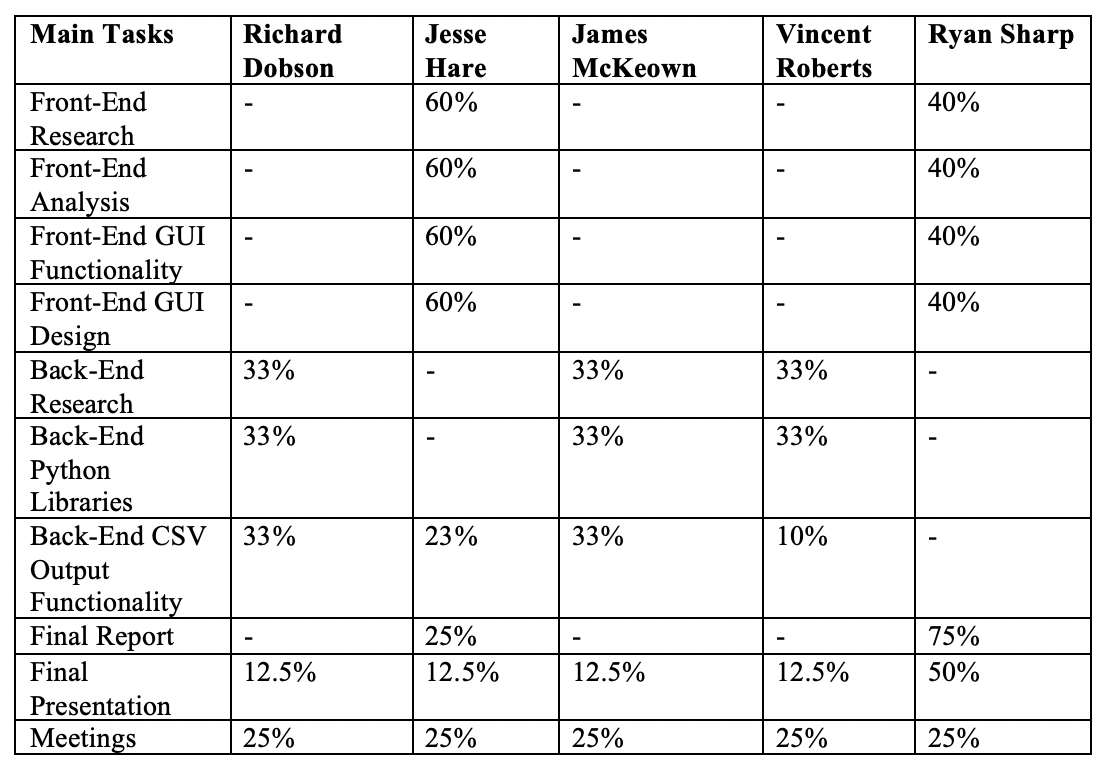
\includegraphics[scale=0.71]{task_distro.png} \\

\newpage


% ----- Section 7 ----- %

\section{7. Conclusions}


\newpage

% ----- Section: Reference List ----- %

\section{Reference List}


\newpage

% ----- Section: Appendix ----- %

\section{Appendix}



\end{document}

